\documentclass[a4paper,11pt,oneside]{article}

\usepackage{amsmath,amssymb,epsfig}
\usepackage{url}
\usepackage[T1]{fontenc}
\usepackage{ae,aecompl}
\usepackage{epsfig}
\usepackage{subfigure}
\addtolength{\voffset}{-1cm}
\addtolength{\hoffset}{-1cm}
\setlength{\parindent}{0in}
\addtolength{\textwidth}{1.8cm}
\addtolength{\textheight}{1cm}
\addtolength{\parskip}{.5cm}

% Example definitions.
% --------------------
\def\x{{\mathbf x}}
\def\X{{\mathbf X}}
\def\u{{\mathbf u}}
\def\U{{\mathbf U}}
\def\x{{\mathbf x}}
\def\s{{\mathbf s}}
\def\A{{\mathbf A}}
\def\y{{\mathbf y}}
\def\W{{\mathbf W}}
\def\w{{\mathbf w}}
\def\B{{\mathbf B}}
\def\a{{\mathbf a}}
\def\D{{\mathbf D}}
\def\P{{\mathbf P}}
\def\n{{\mathbf n}}
\def\V{{\mathbf V}}
\def\R{{\mathbf R}}
\def\I{{\mathbf I}}
\def\M{{\mathbf M}}
\def\sech{{\mathrm{sech}}}
\def\L{{\cal L}}
\def\Cum{{\rm{Cum}}}
\def\var{{\rm{var}}}
\def\T{{\mathbf T}}
\def\C{{\mathbf C}}
\def\tf{{\emph{t-f}}}


% Title.
% ------
\title{\large{\textbf{EXERCISE 3}}}
\author{SGN-1156 Signal Processing Techniques\\
\texttt{http://www.cs.tut.fi/courses/SGN-1156}\\
Tampere University of Technology\\
Germ\'an G\'omez-Herrero, \url{http://germangh.com}}

\date{November 17, 2009}

\begin{document}
\maketitle

\noindent \textbf{PROBLEM 1:} Consider the system of Figure~\ref{fig:fig1a}, where the input unit-energy continuous-time signal $x_{a}(t)$ has a band-limited spectrum $X_{a}(j\Omega)$, as sketched in Figure~\ref{fig:fig1b}, and is being sampled at the Nyquist rate. The discrete-time processor is an ideal lowpass filter with a frequency response $H(e^{j\omega})$, as shown in Figure~\ref{fig:fig1c}, and has a cutoff frequency $\omega_{c}=\Omega_{m}T_{s}/2$ where $T_{s}$ is the sampling period. Sketch as accurately as possible the spectrum $Y_{a}(j\Omega)$ of the output continuous-time signal $y_{a}(t)$. What is the energy of the output signal $y_{a}(t)$?

\begin{figure}[h!]
\centering
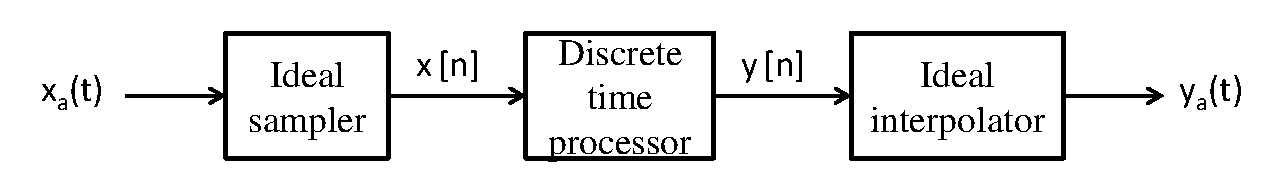
\includegraphics[width=\textwidth]{fig1a.eps}
\caption{Block diagram of the system.}
\label{fig:fig1a}
\end{figure}

\begin{figure}[h!]
\centerline{\subfigure[]{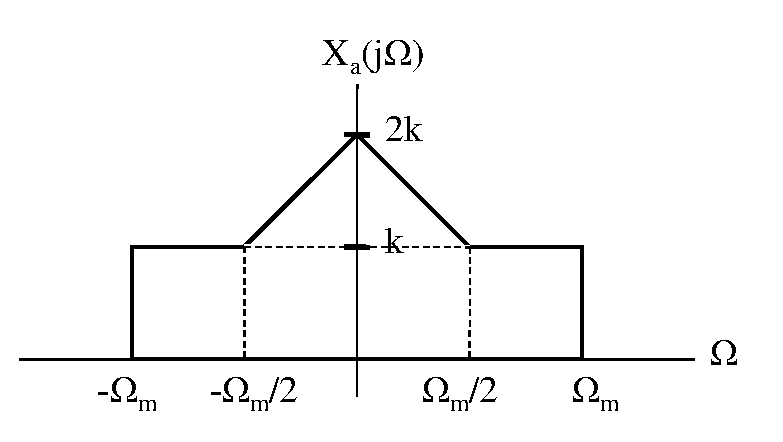
\includegraphics[width=.48\textwidth]{fig1b.eps}
\label{fig:fig1b}
}
\hfil
\subfigure[]{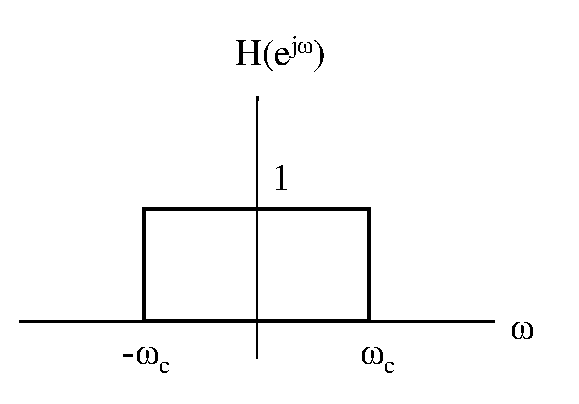
\includegraphics[width=.4\textwidth]{fig1c.eps}\label{fig:fig1c}
}
}
\caption{Spectrum of the input and frequency response of the digital filter. The scalar value $k$ on the left figure is unknown.}
\label{caca}
\end{figure}


\vspace{1cm}

\noindent \textbf{PROBLEM 2:} There is a given signal and noise mixture $x_{a}(t)=s_{a}(t)+\epsilon_{a}(t)$. The signal of interest has a bandwidth of 1000 Hz and the unwanted noise contamination is a sinusoid of frequency equal to 60 Hz, i.e. $\epsilon_{a}(t)=A\sin(120\pi t)$. Design a discrete-time system, which will suppress the noise component $\epsilon_{a}$ in the mixture $x_{a}(t)$. The system should include an ideal A/D converter, a discrete-time filter and an ideal D/A converter. The A/D converter should convert the analog signal into a discrete one $x[n]=x_{a}(nT_{s})$, with an appropriate sampling period $T_{s}$. The discrete-time block should filter out the unwanted noise components by the following difference equation:

\[
y[n]=x[n]+ax[n-1]+bx[n-2]
\]

\noindent Determine the sampling frequency $f_{s}$ of the A/D and D/A converters as well as the parameters $a$ and $b$ of the discrete-time filter.

\vspace{1cm}

\noindent \textbf{PROBLEM 3:} The following \emph{bandpass} signals are to be sampled and fully reconstructed from their sampled versions by using an appropriate bandpass filter. Determine the \emph{smallest possible} sampling frequency $\Omega_{s}$ for each of them, and sketch the frequency response of the reconstruction filters. 

\begin{itemize}
\item[(a)] $x_{a}(t)$ is real, with Fourier transform $X_{a}(j\Omega)$ nonzero for $2\pi \cdot 9000 \leq |\Omega| \leq 2\pi \cdot 12000$.
\item[(b)] $x_{a}(t)$ is real, with Fourier transform $X_{a}(j\Omega)$ nonzero for $2\pi \cdot 18000 \leq |\Omega| \leq 2\pi \cdot 22000$.
\end{itemize}


\vspace{1cm}

\noindent \textbf{PROBLEM 4:} Diagrammed in Figure~\ref{fig:fig3} is a hybrid digital-analog system. The discrete-time system $H_{LPF}(e^{j\omega})$ is a low-pass filter:

\begin{figure}[h!]
\centering
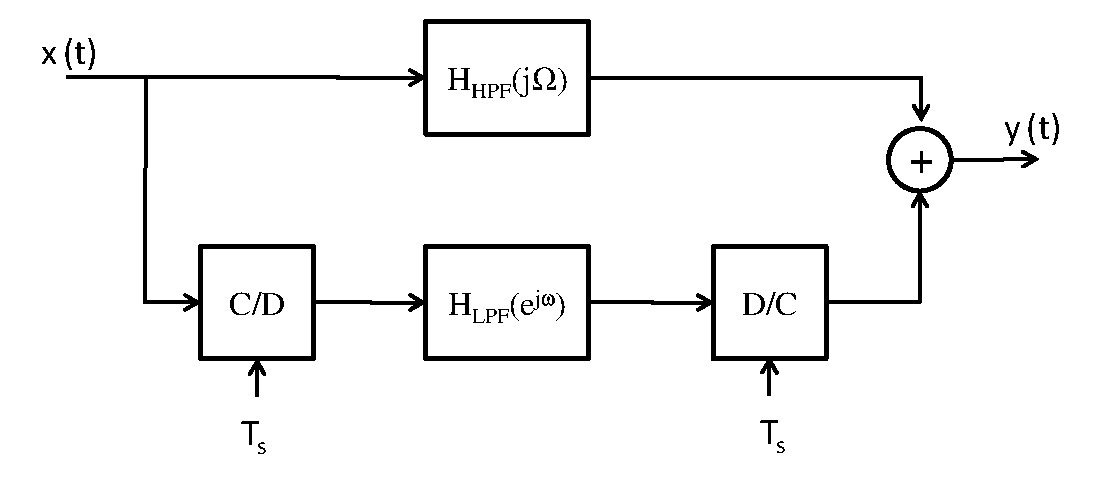
\includegraphics[width=\textwidth]{fig3.eps}
\caption{Hybrid digital-analog system.}
\label{fig:fig3}
\end{figure}

\[
H_{LPF}(e^{j\omega})=\left\{\begin{array}{lll}
A & \qquad &|\omega|\leq \omega_{0}\\
0 & \qquad &\textrm{otherwise}
\end{array}\right.
\]

\noindent and the analog system is a high-pass filter with a frequency response shown in Figure~\ref{fig:fig4}. The input analog signal is bandlimited to $\Omega_{0}=2\pi\cdot 4000$, and the sampling period of the ideal C/D and D/C converters is $T_s=10^{-4}\;s$ Find values for A and $\omega_{0}$ that will result in perfect reconstruction of $x(t)$, i.e. values for which $y(t)=x(t)$.


\begin{figure}[h!]
\centering
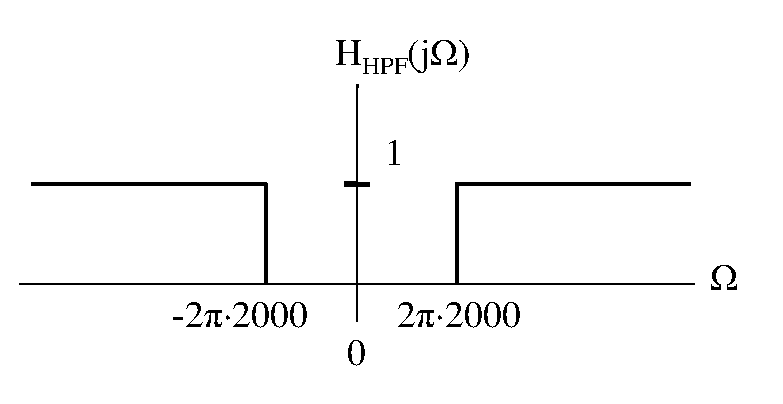
\includegraphics[width=.5\textwidth]{fig4.eps}
\caption{Hybrid digital-analog system.}
\label{fig:fig4}
\end{figure}


\end{document}